\chapter{官能团与类别}\label{ch:g11:functional-groups}

打开一瓶醋、一瓶指甲油去除剂，再拿一袋梨味糖，
再走过鱼贩的摊位：四种气味，分别是刺鼻、甜溶剂味、果香与鱼腥味，
对应四种不同的分子。
每种气味及其化学性质的大部分，并不源于碳骨架，
而源于连在其上的一小群原子：一处是氧与氢，
另一处是一个氮原子。化学家
便依据这些基团对有机化合物分类。

\begin{recall}
键线式、烷烃与烷基的命名、同分异构体
（见\cref{ch:g11:organic-skeletons}）。极性键与氢键
（见\cref{ch:g11:polarity-and-cohesion}）。
\end{recall}

\begin{omfigure}
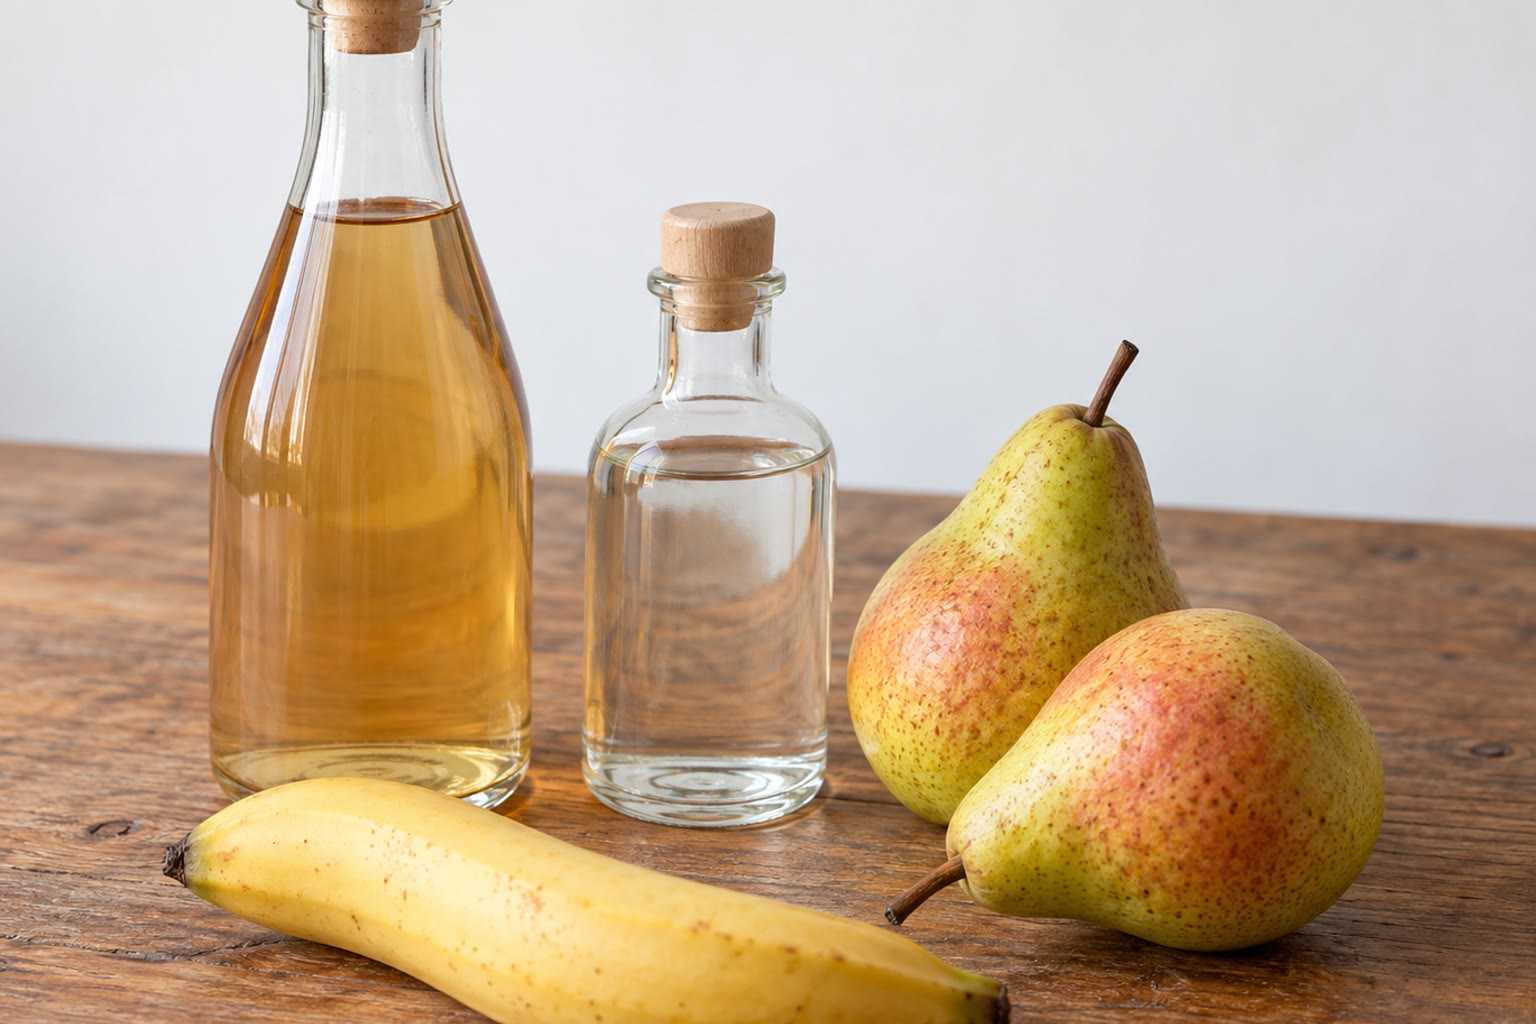
\includegraphics[width=0.5\linewidth]{images/book1/ai/g11-still-life-esters.jpg}

{\small 醋、溶剂与水果：每种气味都来自碳骨架上
不同的一组原子。}
\end{omfigure}

\section{官能团}

\begin{definition}[官能团]\label{def:g11:functional-groups:functional-group}
\emph{官能团}\index{官能团}是指一类原子团，
不包括仅以单键相连的骨架碳原子与氢原子，
它使分子具有特征化学反应。含有同一官能团的
化合物构成一个类别。
\end{definition}

\begin{omfigure}
\renewcommand{\arraystretch}{1.35}
\footnotesize
\begin{tabular}{@{}l@{\enspace}l@{\enspace}l@{\enspace}l@{\enspace}l@{}}
\hline
官能团 & 化学式 & 类别 & 命名 & 例子 \\
\hline
羟基 & \ce{-OH} & 醇 & \emph{某醇} & 乙醇，\ce{CH3-CH2-OH} \\
羰基（端基） & \ce{-CHO} & 醛 & \emph{某醛} & 乙醛，\ce{CH3-CHO} \\
羰基（链中） & \ce{C-CO-C} & 酮 & \emph{某酮} & 丙酮，\ce{CH3-CO-CH3} \\
羧基 & \ce{-COOH} & 羧酸 & \emph{某酸} & 乙酸，\ce{CH3-COOH} \\
酯基 & \ce{C-COO-C} & 酯 & \emph{某酸某酯} & 乙酸乙酯，\ce{CH3-COO-CH2-CH3} \\
胺基 & \ce{-NH2} & 胺 & \emph{某胺} & 乙胺，\ce{CH3-CH2-NH2} \\
酰胺基 & \ce{-CONH2} & 酰胺 & \emph{某酰胺} & 乙酰胺，\ce{CH3-CONH2} \\
卤素 & \ce{C-X} & 卤代烷 & 词头 \emph{氯}，\ldots & 氯甲烷，\ce{CH3Cl} \\
双键 & \ce{C=C} & 烯烃 & \emph{某烯} & 乙烯，\ce{CH2=CH2} \\
\hline
\end{tabular}\par\medskip

\setchemfig{atom sep=1.4em}
\begin{tabular}{@{}c@{\quad}c@{\quad}c@{\quad}c@{\quad}c@{}}
\chemfig{R-C(=[2]O)-H} & \chemfig{R-C(=[2]O)-R'} & \chemfig{R-C(=[2]O)-O-H} &
\chemfig{R-C(=[2]O)-O-R'} & \chemfig{R-C(=[2]O)-N(-[1]H)-[7]H} \\
\small 醛 & \small 酮 & \small 羧酸 & \small 酯 &
\small 酰胺
\end{tabular}\par\medskip

{\small 主要官能团，以及建立在羰基
\ce{C=O} 上的五类官能团，完整画出。R 和 R$'$ 代表碳链（烷基）
和 X 代表卤原子（F、Cl、Br、I）。}
\end{omfigure}

\section{醇及其级数}

\begin{definition}[醇，醇的级数]\label{def:g11:functional-groups:alcohol}
含有羟基 \ce{-OH} 且连于只含单键的碳原子上的化合物，称为\emph{醇}\index{醇}。
\emph{醇的级数}\index{醇的级数}由连有 \ce{-OH} 的碳原子
所连接的其他碳原子数决定：连接一个、两个或三个时，
分别为伯醇、仲醇或叔醇。（甲醇 \ce{CH3OH}
中的碳原子不与其他碳原子相连，
也计入伯醇。）
\end{definition}

\begin{omfigure}
\setchemfig{atom sep=1.9em}
\begin{tabular}{ccc}
\chemfig{-[:30]-[:-30]-[:30]-[:-30]OH} &
\chemfig{-[:30](-[:90]OH)-[:-30]-[:30]} &
\chemfig{-[:0](-[:90]OH)(-[:-90])-[:0]} \\[4pt]
\small 1-丁醇 & \small 2-丁醇 & \small 2-甲基-2-丙醇 \\
\small \textbf{伯醇} & \small \textbf{仲醇} & \small \textbf{叔醇} \\
\small （与 \ce{-OH} 相连的碳：1 个碳邻居） & \small （2 个邻居） &
\small （3 个邻居）
\end{tabular}

{\small 三种同分异构体 \ce{C4H10O}，对应三种级数的醇。}
\end{omfigure}

\section{醛、酮、酸和酯}

\begin{definition}[醛、酮]\label{def:g11:functional-groups:carbonyl}
羰基是 \ce{C=O} 双键。若羰基碳原子位于链端（与至少一个氢原子相连），
则该化合物为\emph{醛}\index{醛}；
若羰基碳原子位于链中（与两个碳原子相连），
则该化合物为\emph{酮}\index{酮}。
\end{definition}

\begin{definition}[羧酸、酯]\label{def:g11:functional-groups:carboxylic-acid}
\emph{羧酸}\index{羧酸}含有羧基 \ce{-COOH}，
其中碳原子同时连有羰基和羟基。\emph{酯}\index{酯}含有
\ce{-COO-} 基团，位于两个碳链之间；
它可看作由酸的 \ce{-OH} 被来自醇的
\ce{-O-}R$'$ 取代得到。
\end{definition}

\begin{example}[乙酸乙酯]\label{ex:g11:functional-groups:ethyl-ethanoate}
溶剂乙酸乙酯 \ce{CH3-COO-CH2-CH3} 带有梨味糖
和指甲油去除剂的气味。它的“酸部分”\ce{CH3-CO}，
来自乙酸 \ce{CH3-COOH}，给出名称中的
\emph{乙酸}一词；它的“醇部分”\ce{O-CH2-CH3}，
来自乙醇 \ce{CH3-CH2-OH}，给出名称中的\emph{乙基}一词。在后面一章中
将说明酯如何由酸和醇制得。
\end{example}

\begin{omfigure}
\setchemfig{atom sep=2.2em}
\chemfig{@{a}H_3C-@{c}C(=[2]@{o}O)-@{x}O-CH_2-@{z}CH_3}
\chemmove{
  \fill[omProp, opacity=0.14, rounded corners]
    ($(a.south west)+(-0.12,-0.15)$) rectangle ($(o.north east)+(0.25,0.12)$);
  \fill[omDef, opacity=0.14, rounded corners]
    ($(x.south west)+(-0.2,-0.15)$) rectangle ($(z.north east)+(0.4,0.75)$);
  \node[omProp, anchor=north east, align=right, font=\small] at ($(c.south)+(0.15,-0.25)$)
    {酸部分，来自乙酸：\\ \emph{乙酸}};
  \node[omDef, anchor=north west, align=left, font=\small] at ($(x.south)+(0.05,-0.25)$)
    {醇部分，来自乙醇：\\ \emph{乙基}};}
\par\vspace{1.4cm}

{\small 酯的命名：酸部分给出酸名
（\emph{乙酸}），醇部分的烷基名称（\emph{乙基}）
改为“某酯”（\emph{乙酯}）；名称为“乙酸乙酯”。}
\end{omfigure}

\section{胺、酰胺、卤代烷和烯烃}


\begin{definition}[胺、酰胺]\label{def:g11:functional-groups:amine}
氮原子通过单键与碳链相连的结构称为\emph{胺}\index{胺}，
如 \ce{-NH2}。\emph{酰胺}\index{酰胺}是氮原子
与羰基中的碳原子相连的结构，如 \ce{-CO-NH2}。
\end{definition}

\begin{definition}[卤代烷、烯烃]\label{def:g11:functional-groups:halogenoalkane}
\emph{卤代烷}\index{卤代烷}是烷烃中
一个或多个氢原子被卤素原子（F、Cl、Br、I）取代后的产物。
\emph{烯烃}\index{烯烃}含有碳碳双键，即 \ce{C=C}。
\end{definition}

\begin{remark}[气味与官能团]\label{rem:g11:functional-groups:smells}
许多小分子的胺带有腐鱼的气味，不新鲜的鱼的气味
主要由它们造成。许多小分子的酯带有水果香味。
小分子羧酸的气味刺鼻，如同醋；丙酮是一种酮，
其气味正是人们熟悉的指甲油去除剂的气味。
\end{remark}

\section{命名}

\begin{method}[命名含单一官能团的有机化合物]\label{met:g11:functional-groups:naming}
\begin{enumerate}
  \item 找出最长的、\emph{包含}官能团碳原子的碳链
        （对醇或胺而言，则是带有该官能团的碳原子），
        它给出词根。
  \item 对碳链编号，从使官能团位次
        最低的一端开始。
  \item 将烷烃的\emph{-e}替换为所属类别的词尾，
        必要时在词尾前加上官能团的位次，如丙-2-醇、
        丁-2-酮。（醛、羧酸和酰胺的官能团位于 1 号碳上，
        不必标注位次。）
  \item 将烷基取代基作为词头加上，并标明位次，
        与烷烃的命名相同；卤素总是作为词头，如 2-氯丙烷。
\end{enumerate}
\end{method}

\begin{example}[四个名称]\label{ex:g11:functional-groups:names}
\setchemfig{atom sep=1.7em}
\chemfig{-[:30](-[:90]OH)-[:-30]} 是丙-2-醇（仲醇）；
\chemfig{-[:30](=[:90]O)-[:-30]-[:30]} 是丁-2-酮；
\chemfig{-[:30]-[:-30]-[:30](=[:90]O)-[:-30]OH} 是丁酸；
\chemfig{-[:30](-[:90])-[:-30]-[:30]=[:-30]O} 是 3-甲基丁醛。
\end{example}

\begin{omfigure}
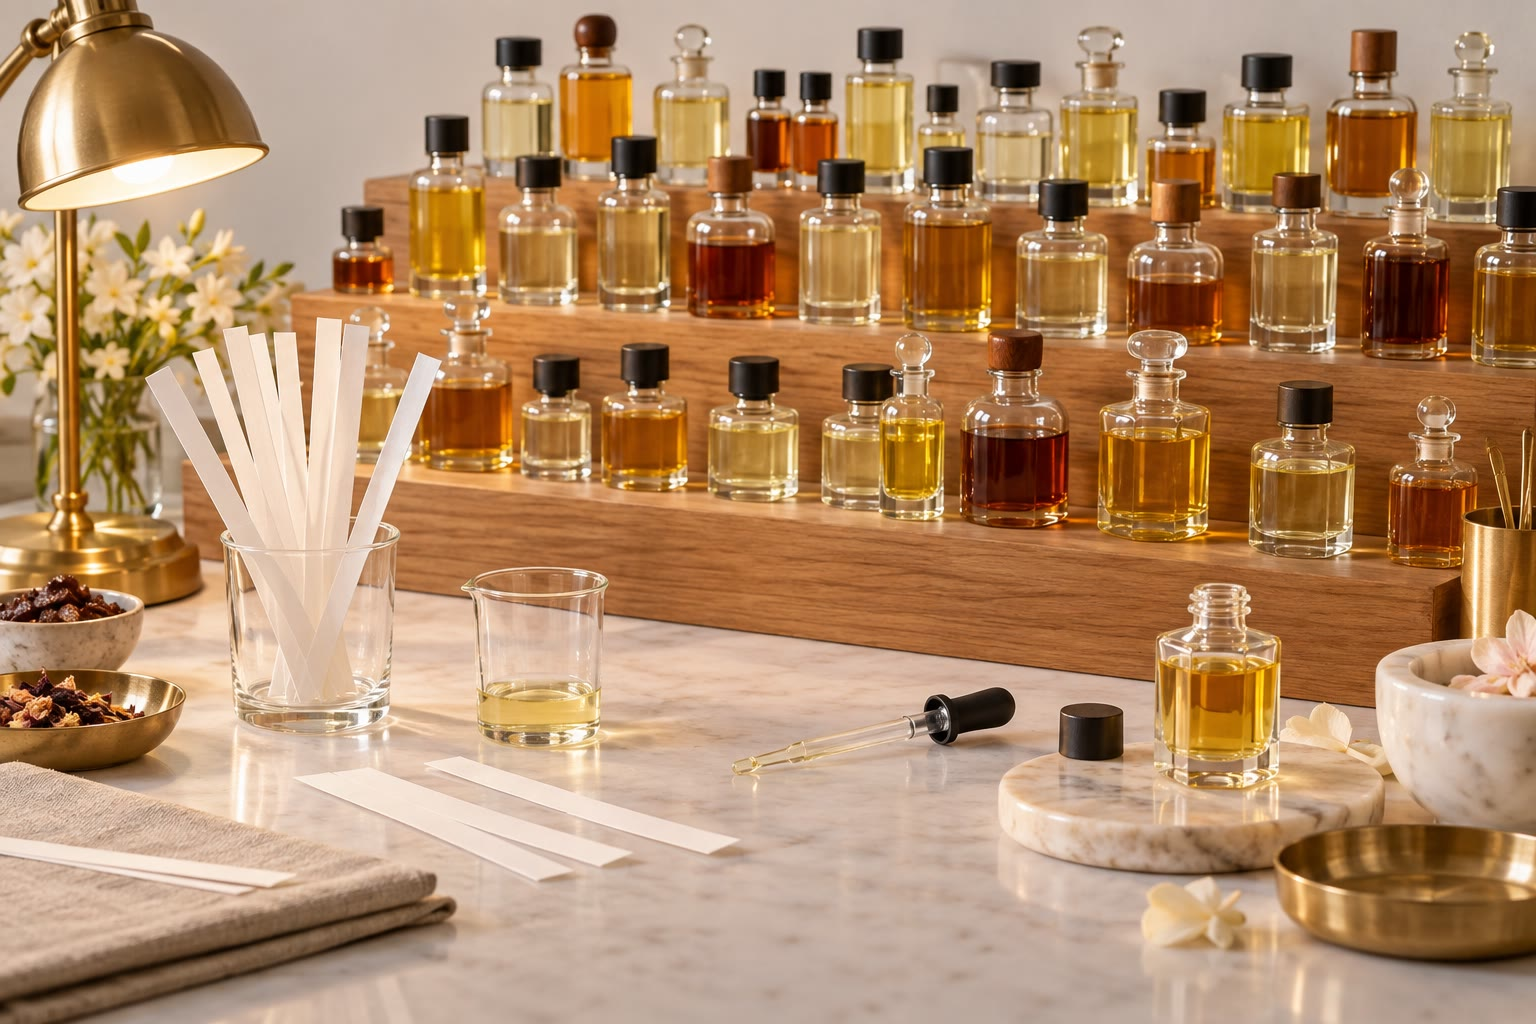
\includegraphics[width=0.48\linewidth]{images/book1/ai/g11-perfumer-lab.jpg}

{\small 调香师的工作台：许多瓶子里装有酯、醇、
醛和酮。}
\end{omfigure}

\begin{safety}{\ghs[0.82cm]{GHS02}\ghs[0.82cm]{GHS05}\ghs[0.82cm]{GHS07}}
% ledger: ghs:acetone, ghs:acetic-acid
丙酮高度易燃，并刺激眼睛；其蒸气
会使人昏昏欲睡。纯乙酸易燃，并会造成
严重的皮肤和眼睛灼伤；醋是它的稀溶液。
检验气味绝不可直接对着烧瓶嗅闻：应用手将蒸气
轻轻扇向鼻部，且仅在教师
指示时方可这样做。
\end{safety}

\section{练习}


\begin{exercise}[$\star$]\label{exo:g11:functional-groups:1}
指出下列各化合物的官能团及所属类别：
\ce{CH3-CH2-CH2-OH}; \ce{CH3-CO-CH2-CH3}; \ce{CH3-CH2-COOH};
\ce{CH3-COO-CH3}; \ce{CH3-CH2-NH2}.
\end{exercise}

\begin{exercise}[$\star$]\label{exo:g11:functional-groups:2}
写出下列化合物的名称：\ce{CH3-OH}；\ce{CH3-CH2-CH2-OH}；\ce{HCOOH}；\ce{CH3-CH2-CHO}；
\ce{CH3-CO-CH3}.
\end{exercise}

\begin{exercise}[$\star$]\label{exo:g11:functional-groups:3}
下列各化合物分别属于哪一类：丁-2-醇、戊醛、丙酸
甲酯、丙酰胺、2-溴丙烷、丁-1-烯？
\end{exercise}

\begin{exercise}[$\star$]\label{exo:g11:functional-groups:4}
写出丙醛和丙酮的结构简式。哪一种
是醛？你如何判断？
\end{exercise}

\begin{exercise}[$\star$]\label{exo:g11:functional-groups:5}
指出丙-1-醇、丙-2-醇和 2-甲基丙-2-醇的醇级数。
\end{exercise}

\begin{exercise}[$\star\star$]\label{exo:g11:functional-groups:6}
画出戊-3-醇、2-甲基丁酸、
己-2-酮和乙酸丙酯的键线式。
\end{exercise}

\begin{exercise}[$\star\star$]\label{exo:g11:functional-groups:7}
丙醛和丙酮具有相同的分子式。写出该分子式。它们是否
互为同分异构体？它们含有相同的官能团吗？
\end{exercise}

\begin{exercise}[$\star\star$]\label{exo:g11:functional-groups:8}
写出酯的结构简式和名称，该酯的酸部分来自甲酸
\ce{HCOOH}，醇部分来自乙醇；再写出由乙酸和丙-1-醇生成的
酯的结构简式和名称。
\end{exercise}

\begin{exercise}[$\star\star$]\label{exo:g11:functional-groups:9}
命名下列酯 \ce{CH3-COO-CH3}、\ce{CH3-CH2-COO-CH2-CH3} 和
\ce{HCOO-CH3}，并指出每种酯分别与哪种酸和哪种醇相关。
\end{exercise}

\begin{exercise}[$\star\star$]\label{exo:g11:functional-groups:10}
画出并命名分子式为 \ce{C4H10O} 的四种醇，
并指出每种醇的级数。
\end{exercise}

\begin{exercise}[$\star\star$]\label{exo:g11:functional-groups:11}
利用族表，\ce{CH3-CO-NH2} 属于哪一族？
烯烃的名称以什么词尾结尾？哪些族的
羰基碳原子上同时连有氧原子或氮原子？
\end{exercise}

\begin{exercise}[$\star\star\star$]\label{exo:g11:functional-groups:12}
圈出阿司匹林和对乙酰氨基酚中的官能团，并命名。
（像对乙酰氨基酚中那样直接连在环上的 \ce{-OH} 称为
酚羟基，它的性质与醇不同。）
\begin{center}
\setchemfig{atom sep=1.6em}
\chemfig{*6(-=-(-COOH)=(-O-[:150]C(=[:90]O)-[:210]H_3C)-=)}
\qquad
\chemfig{*6((-OH)=-=(-N(-[2]H)-[7]C(=[6]O)-[1]CH_3)-=-)}
=\\[2pt] \small 阿司匹林 \hspace{4.2cm} 对乙酰氨基酚
\end{center}
\end{exercise}

\begin{exercise}[$\star\star\star$]\label{exo:g11:functional-groups:13}
% ledger: bp:C2H5OH, bp:CH3OCH3
乙醇 \ce{CH3-CH2-OH} 和甲醚 \ce{CH3-O-CH3} 具有相同的
分子式。写出该分子式。甲醚属于表中未列出的
醚类。两者中哪一种分子之间能形成氢键？
哪一种的沸点更高（一种为 \qty{78}{\celsius}，
另一种为 \qty{-25}{\celsius}）？
\end{exercise}

\begin{exercise}[$\star\star\star$]\label{exo:g11:functional-groups:14}
乳酸由疲劳的肌肉产生，其结构为
\chemfig{CH_3-CH(-[2]OH)-COOH}。命名其中的两种官能团。当分子中既有羧基又有其他基团时，
羧酸作为母体，其他基团作为词头，
（\emph{羟基-}对应 \ce{-OH}，
\emph{氨基-}对应 \ce{-NH2}）。命名乳酸，再命名甘氨酸
\ce{H2N-CH2-COOH}。
\end{exercise}

\begin{exercise}[$\star\star\star$]\label{exo:g11:functional-groups:15}
敞口放置于空气中的葡萄酒会变成醋：乙醇经
乙醛被氧化为乙酸。写出这三种化合物的结构简式和分子式，
并指出它们所属的类别。每一步中，分子式
发生了什么变化？
\end{exercise}

\section{问题：水果香味}

\begin{problem}[{周末问题——一位香料化学家合成香蕉的
香味：关键分子的摩尔质量是多少？}]
\label{pb:g11:functional-groups:1}
% ledger: aw:C, aw:H, aw:O
一位香料化学家的工作台上有五种化合物：
\begin{center}
\begin{tabular}{ll}
A & \chemfig{CH_3-C(=[2]O)-O-CH_2-CH_2-CH(-[2]CH_3)-CH_3} \\[16pt]
B & \chemfig{HO-CH_2-CH_2-CH(-[2]CH_3)-CH_3} \\[10pt]
C & \ce{CH3-COOH} \\
D & \ce{CH3-CH2-CH2-CH2-CH2-CHO} \\
E & \ce{CH3-CH2-CH2-COO-CH2-CH3}
\end{tabular}
\end{center}
A 带有香蕉和梨糖的香气，B 带有麦芽的香气，C 带有醋味，D 带有
刚割青草的气味，E 带有菠萝的香气。

\medskip
\noindent\textbf{第一部分——官能团与类别。}
\begin{enumerate}
  \item 命名每种化合物的官能团。
  \item 指出每种化合物所属的类别。
  \item 哪些化合物是酯？它们各有什么香味？
  \item 醇 B 的级数是多少？
  \item 写出 D 的分子式，并画出 D 的
        一种酮类同分异构体。
\end{enumerate}

\medskip
\noindent\textbf{第二部分——命名。}
\begin{enumerate}[resume]
  \item 命名 B（找出连有 \ce{-OH} 的碳原子所在的
        最长碳链）。
  \item 命名 C 和 D。
  \item 命名 E，并指出它与哪种酸和哪种醇相关。
  \item 解释 A 的名称 3-甲基丁基乙酸酯：其中哪一部分来自酸，
        哪一部分来自醇？
\end{enumerate}

\medskip
\noindent\textbf{第三部分——由酸和醇生成。}
\begin{enumerate}[resume]
  \item A 与工作台上的哪两种化合物相关？
  \item 写出 A、B 和 C 的分子式。
  \item 酯由其酸和醇脱去一个小分子生成，
        利用分子式判断脱去的是哪种小分子。
  \item 用分子式写出 A 生成的方程式，
        并检验其是否配平。
\end{enumerate}

\medskip
\noindent\textbf{第四部分——摩尔质量。}
\begin{enumerate}[resume]
  \item 计算 B 和 C 的摩尔质量。
  \item 由第 13 题的方程式推出 A 的摩尔质量。
  \item 直接由 A 的分子式计算其摩尔质量，
        并加以比较。
  \item 某一未知果味样品的摩尔质量接近
        \qty{116}{g/mol}。它是 A 还是 E？
  \item 庚酸 \ce{CH3-(CH2)5-COOH} 有哈喇味。证明它是
        A 的同分异构体。仅凭摩尔质量能否确定一种化合物？
  \item 化学家为什么说，气味既取决于官能团，
        也取决于骨架？以 A 和庚酸为例说明。
  \item 给出最终答案：香蕉酯 3-甲基丁基乙酸酯的
        摩尔质量是多少？
\end{enumerate}
\end{problem}
